\section{Finding 16 - Vulnerable Software leads to Remote Code Execution}

%center under chapter title a one row table with 6 coloumns and no borders
\vspace*{-0,3cm}
\begin{center}
    \begin{tabular}{c c c c}
        \textbf{Classification:} & Remote Code Execution & \textbf{Severity:} & \textbf{\textcolor{red}{High}}  
        \end{tabular}
\end{center}
A vulnerable compiled python script named ”check\_version.pyc” is located in the directory ”usr/local/bin”.

\subsection{Finding Impact}
The vulnerability in this script allows an attacker to execute arbitrary code on the \ac{DUT}. The script sends a GET request to the URL ”https://dhbw.johannes-bauer.com/offsec/”. Included in the GET request the script sends the MAC-Address of the \ac{DUT} as an argument within the URL. If the responds to that request with a HTTP status code of 200, the script executes the responses arguments in a shell on the \ac{DUT}.
It seems like the wanted purpose is to execute the following command on the \ac{DUT} in a subprocess:
\begin{lstlisting}[language=bash]
    $ ip link show eth0
\end{lstlisting}
This command shows the MAC-Address of the network interface ”eth0” on the \ac{DUT}. This MAC-Address is then sent to the server within the GET request (/mac=MAC-Address). The servers response is then executed on the \ac{DUT} and the output is sent back to server again encoded in base64.
An attacker could use this vulnerability to send a carefully crafted response to the \ac{DUT} which executes arbitrary code on the \ac{DUT}.
\subsection{Finding Details}
The decompiled ”check\_version.pyc” script can be found in the appendix.
While testing the python script was executed to get a look at Wireshark but the output couldn't be interpreted. The \ac{DUT} is definitely trying to reach the server but then Wireshark shows that the TCP Port numbers are reused:
%image
\begin{figure}[h]
    \centering
    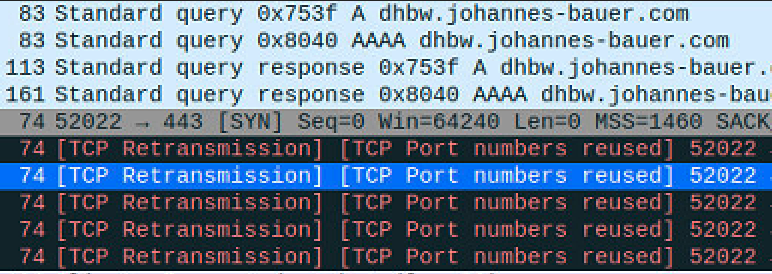
\includegraphics[width=0.8\textwidth]{img/wshk_screen.png}
    \caption{Screenshot of Wireshark}
    \label{fig:fin11}
\end{figure}
\subsection{Evaluation of Results}
\begin{center}
    \begin{tabular}{cccc}
    \textbf{Effort to Fix:} & &\ \textbf{\textcolor{orange}{Medium}}\
    \end{tabular}
\end{center}
How do you judge the individual technical findings (severity, likelihood)?
What is your suggested remediation, if there is one?
How can the customer validate their remediation is effective once implemented?